\documentclass[tikz,border=2pt]{standalone}

\usepackage{pgfplots}
\pgfplotsset{compat=1.18}

\begin{document}
	
	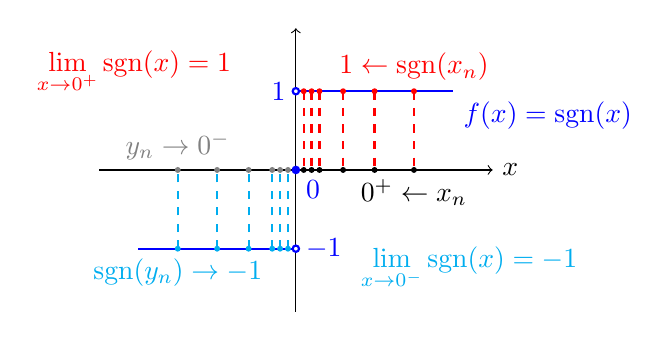
\begin{tikzpicture}[scale=1]
		% Draw axes
		\draw [->] (-2.5,0) -- (2.5,0) node [right] {$x$};
		\draw [->] (0,-1.8) -- (0,1.8);
		% Draw function
		\draw [blue, thick] (-2,-1) -- (0,-1) node [right] {$-1$};
		\draw (-0.7,0.85) node [red, above left] {$\lim\limits_{x\to 0^+}\mathrm{sgn}(x)=1$};
		\draw (0.7,-0.85) node [cyan, below right] {$\lim\limits_{x\to 0^-}\mathrm{sgn}(x)=-1$};
		\draw [blue, thick] (0,1) node [left] {$1$} -- (2,1)  node [below right] {$f(x)=\mathrm{sgn}(x)$};
		\draw [blue, thick, fill=blue] (0,0) circle [radius=0.04] node [below right] {$0$};
		\draw [blue, thick, fill=white] (0,1) circle [radius=0.04];
		\draw [blue, thick, fill=white] (0,-1) circle [radius=0.04];
		% Draw sequences
		\draw [gray,fill=gray] (-1.5,0) circle [radius=0.03] node [above]{$y_n\to 0^-$};
		\draw [gray,fill=gray] (-1,0) circle [radius=0.03];
		\draw [gray,fill=gray] (-0.6,0) circle [radius=0.03];
		\draw [gray,fill=gray] (-0.3,0) circle [radius=0.03];
		\draw [gray,fill=gray] (-0.2,0) circle [radius=0.03];
		\draw [gray,fill=gray] (-0.1,0) circle [radius=0.03];
		\draw [black,fill=black] (1.5,0) circle [radius=0.03] node [below]{$0^+ \leftarrow x_n$};
		\draw [black,fill=black] (1,0) circle [radius=0.03] ;
		\draw [black,fill=black] (0.6,0) circle [radius=0.03];
		\draw [black,fill=black] (0.3,0) circle [radius=0.03];
		\draw [black,fill=black] (0.2,0) circle [radius=0.03];
		\draw [black,fill=black] (0.1,0) circle [radius=0.03];
		
		\draw [cyan,fill=cyan] (-1.5,-1) circle [radius=0.03];
		\draw [cyan,fill=cyan] (-1,-1) circle [radius=0.03];
		\draw [cyan,fill=cyan] (-0.6,-1) circle [radius=0.03];
		\draw [cyan,fill=cyan] (-0.3,-1) circle [radius=0.03];
		\draw [cyan,fill=cyan] (-0.2,-1) circle [radius=0.03];
		\draw [cyan,fill=cyan] (-0.1,-1) circle [radius=0.03];
		\draw [red,fill=red] (1.5,1) circle [radius=0.03];
		\draw [red,fill=red] (1,1) circle [radius=0.03];
		\draw [red,fill=red] (0.6,1) circle [radius=0.03];
		\draw [red,fill=red] (0.3,1) circle [radius=0.03];
		\draw [red,fill=red] (0.2,1) circle [radius=0.03];
		\draw [red,fill=red] (0.1,1) circle [radius=0.03];
		
		\draw [cyan, thick, dashed] (-1.5,-1) node [below]{$\mathrm{sgn}(y_n)\to -1$} -- (-1.5,0);
		\draw [cyan, thick, dashed] (-1,-1) -- (-1,0);
		\draw [cyan, thick, dashed] (-0.6,-1) -- (-0.6,0);
		\draw [cyan, thick, dashed] (-0.3,-1) -- (-0.3,0);
		\draw [cyan, thick, dashed] (-0.2,-1) -- (-0.2,0);
		\draw [cyan, thick, dashed] (-0.1,-1) -- (-0.1,0);
		
		\draw [red, thick, dashed] (1.5,1) node [above]{$1\leftarrow \mathrm{sgn}(x_n)$} -- (1.5,0);
		\draw [red, thick, dashed] (1,1) -- (1,0);
		\draw [red, thick, dashed] (0.6,1) -- (0.6,0);
		\draw [red, thick, dashed] (0.3,1) -- (0.3,0);
		\draw [red, thick, dashed] (0.2,1) -- (0.2,0);
		\draw [red, thick, dashed] (0.1,1) -- (0.1,0);
	\end{tikzpicture}
	
\end{document}